\documentclass{article}

\usepackage{amsmath}
\usepackage{amsthm}
\usepackage{amsfonts}
\usepackage{framed}

%% Simple AMSthm environments, numbered together.
\newtheorem{lem}{Lemma}
\newtheorem{thm}[lem]{Theorem}
\newtheorem{conj}[lem]{Conjecture}

\theoremstyle{definition}
\newtheorem{defn}[lem]{Definition}

\begin{document}

\begin{framed}
  Make sure to explain assumptions you make about the code you
  analyze. For instance, for pointer analysis, you may have made some
  assumptions about the aliasing information known about input
  parameters. Explain those assumptions and why they are reasonable.

  Part of this project is to come up with a useful set of benchmarks
  on which to test and improve your analysis. Discuss why you chose
  those benchmarks, and what makes them interesting. If your
  implementation fails on some benchmarks (there's no shame in it!),
  then explain why and how the analysis might be improved.
\end{framed}

The difficulty of getting the various analyses to work properly on a
piece of code is tightly coupled with the complexity of the underlying
control flow graph. Pathologies that underly implementations of flow
functions may not arise in straight-line programs but become painfully
obvious when branches are introduced. Our benchmarks are designed to
illustrate that our analyses are robust to non-trivial control flow
structures.

Broadly speaking, we have three types of benchmark. The first type is
straight-line programs, which introduce no branches in control
structure. They are the easiest to handle, and our analyses are
accordingly precise on them. Simple branching programs are the second
type, and they introduce conditional branches into fold, but do not
exhibit loops. They are slightly more challenging, but SSA makes them
much easier to handle. Our final type of benchmark is looping
programs. As their name suggests, they have loops, which makes
precision quite difficult.

\subsection{Benchmarks/Assumptions in Common}
Because we have a common pool of benchmarks, we can list them here
along with common assumptions on code. More specialized discussion of
per-analysis benchmark goes below. Here, we can also introduce the
Straight Line Program/Branching Program distinction.

\subsection{Constant Propagation}
\subsection{Available Expressions}
A straight line program where we can do CSE:
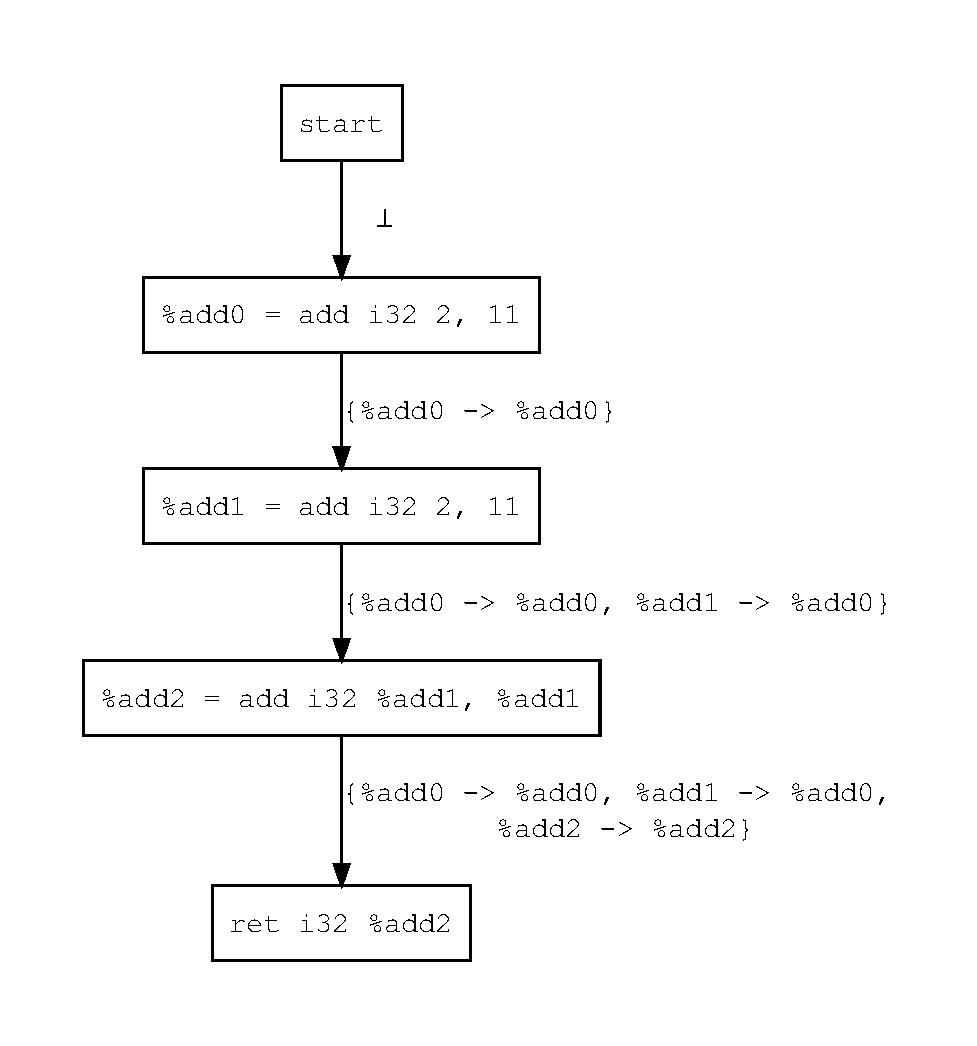
\includegraphics[scale=.4]{figures/cse/straight-line/can-do.pdf}
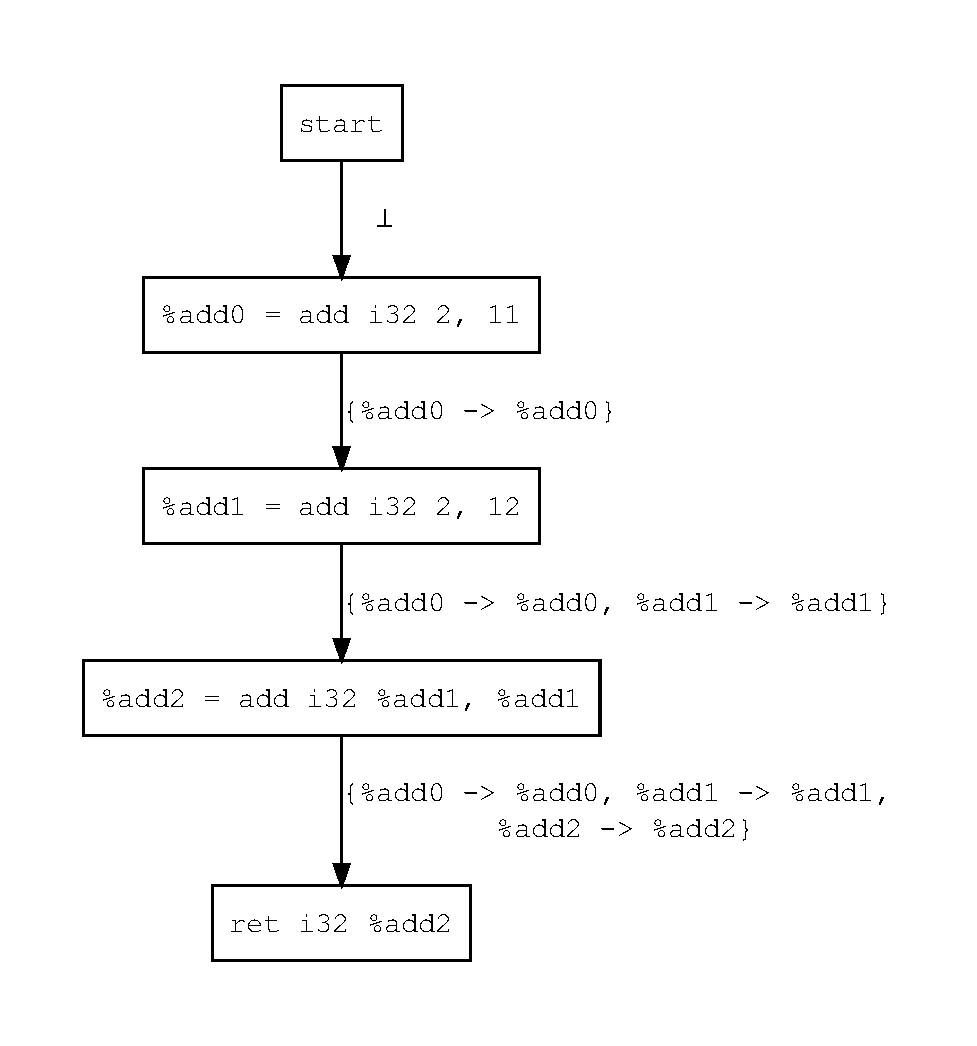
\includegraphics[scale=.4]{figures/cse/straight-line/no-do.pdf}
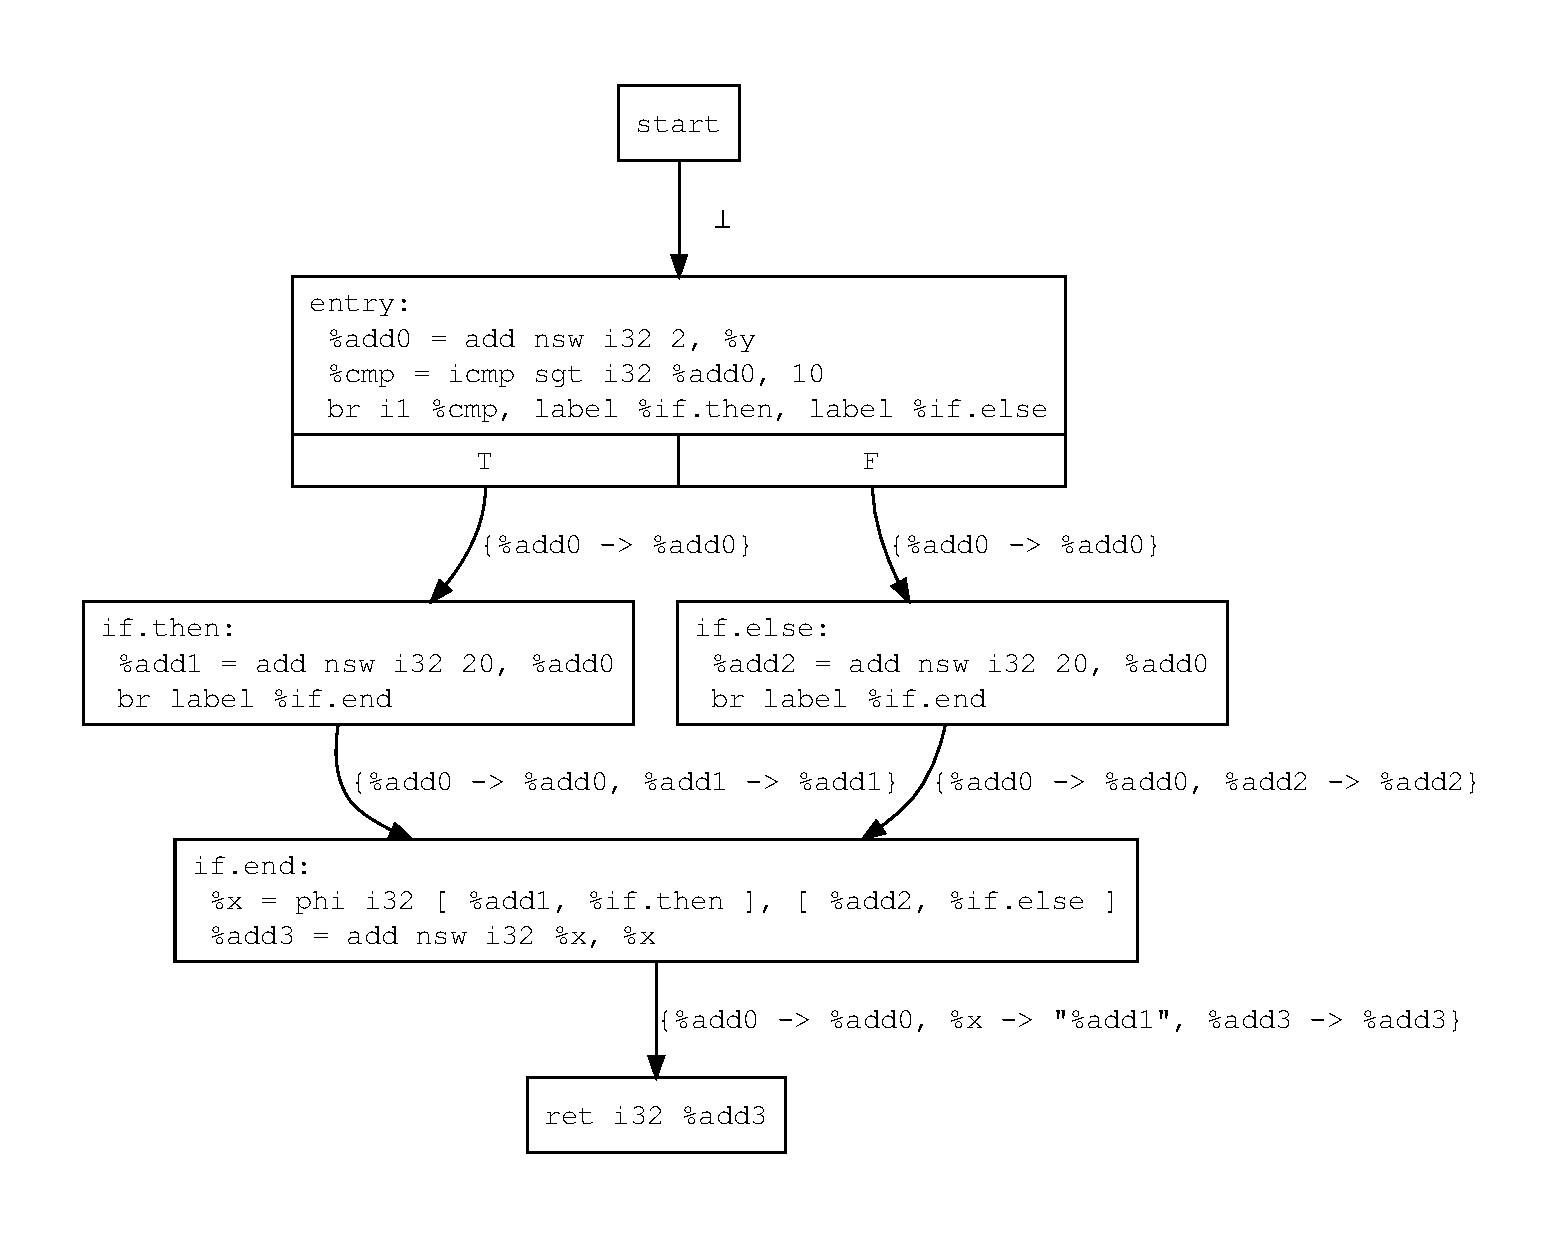
\includegraphics[scale=.4]{figures/cse/branch/can-do-cse.pdf}
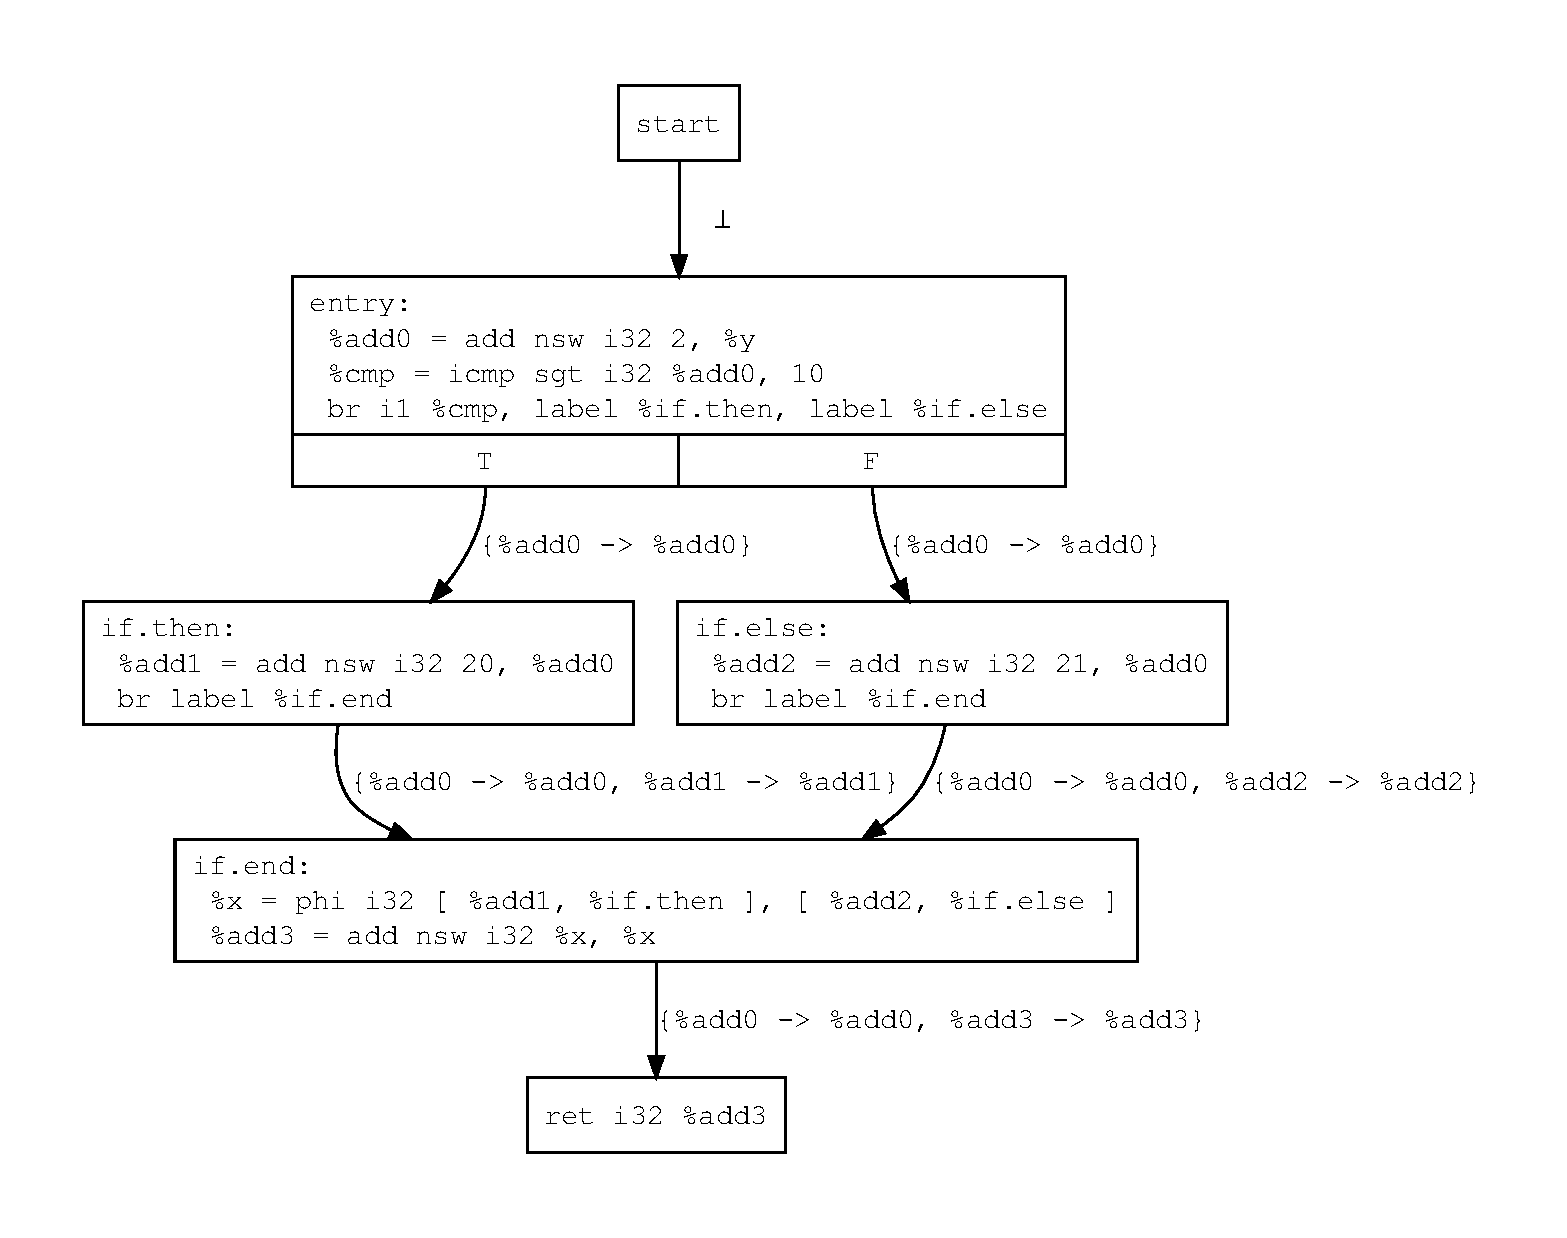
\includegraphics[scale=.4]{figures/cse/branch/no-do.pdf}
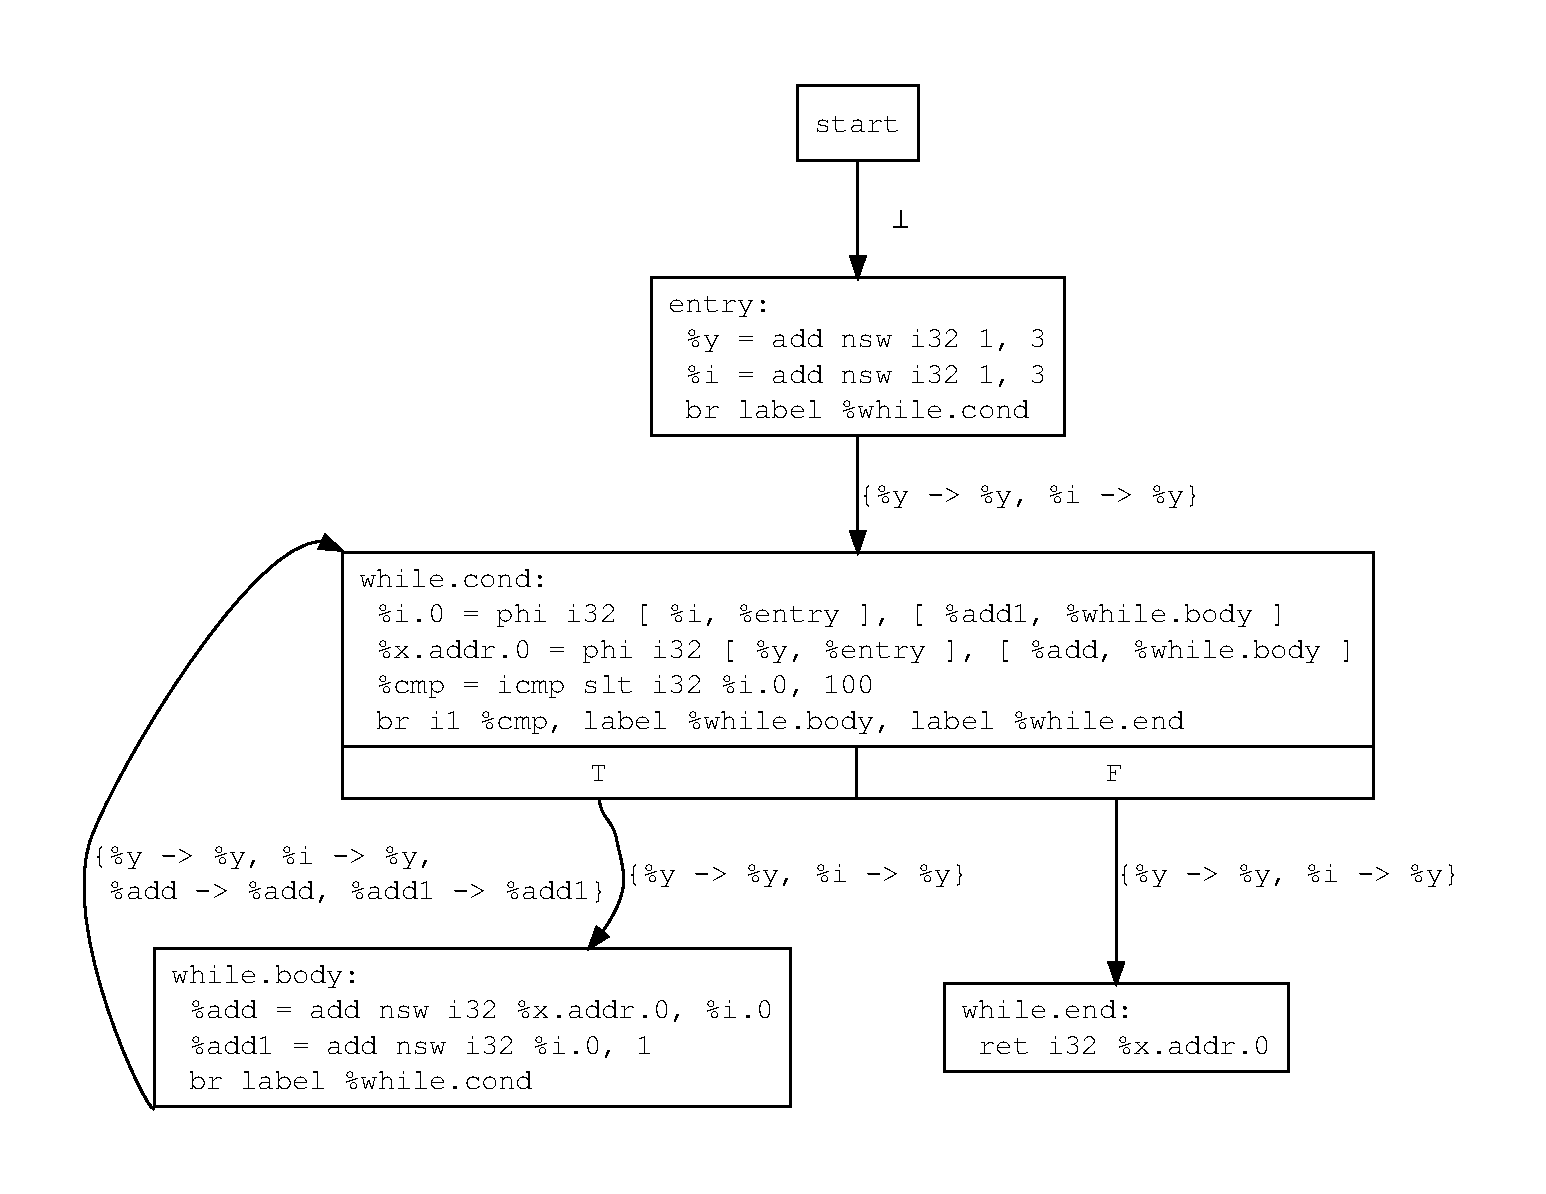
\includegraphics[scale=.4]{figures/cse/loop/loop-can-do-cse.pdf}
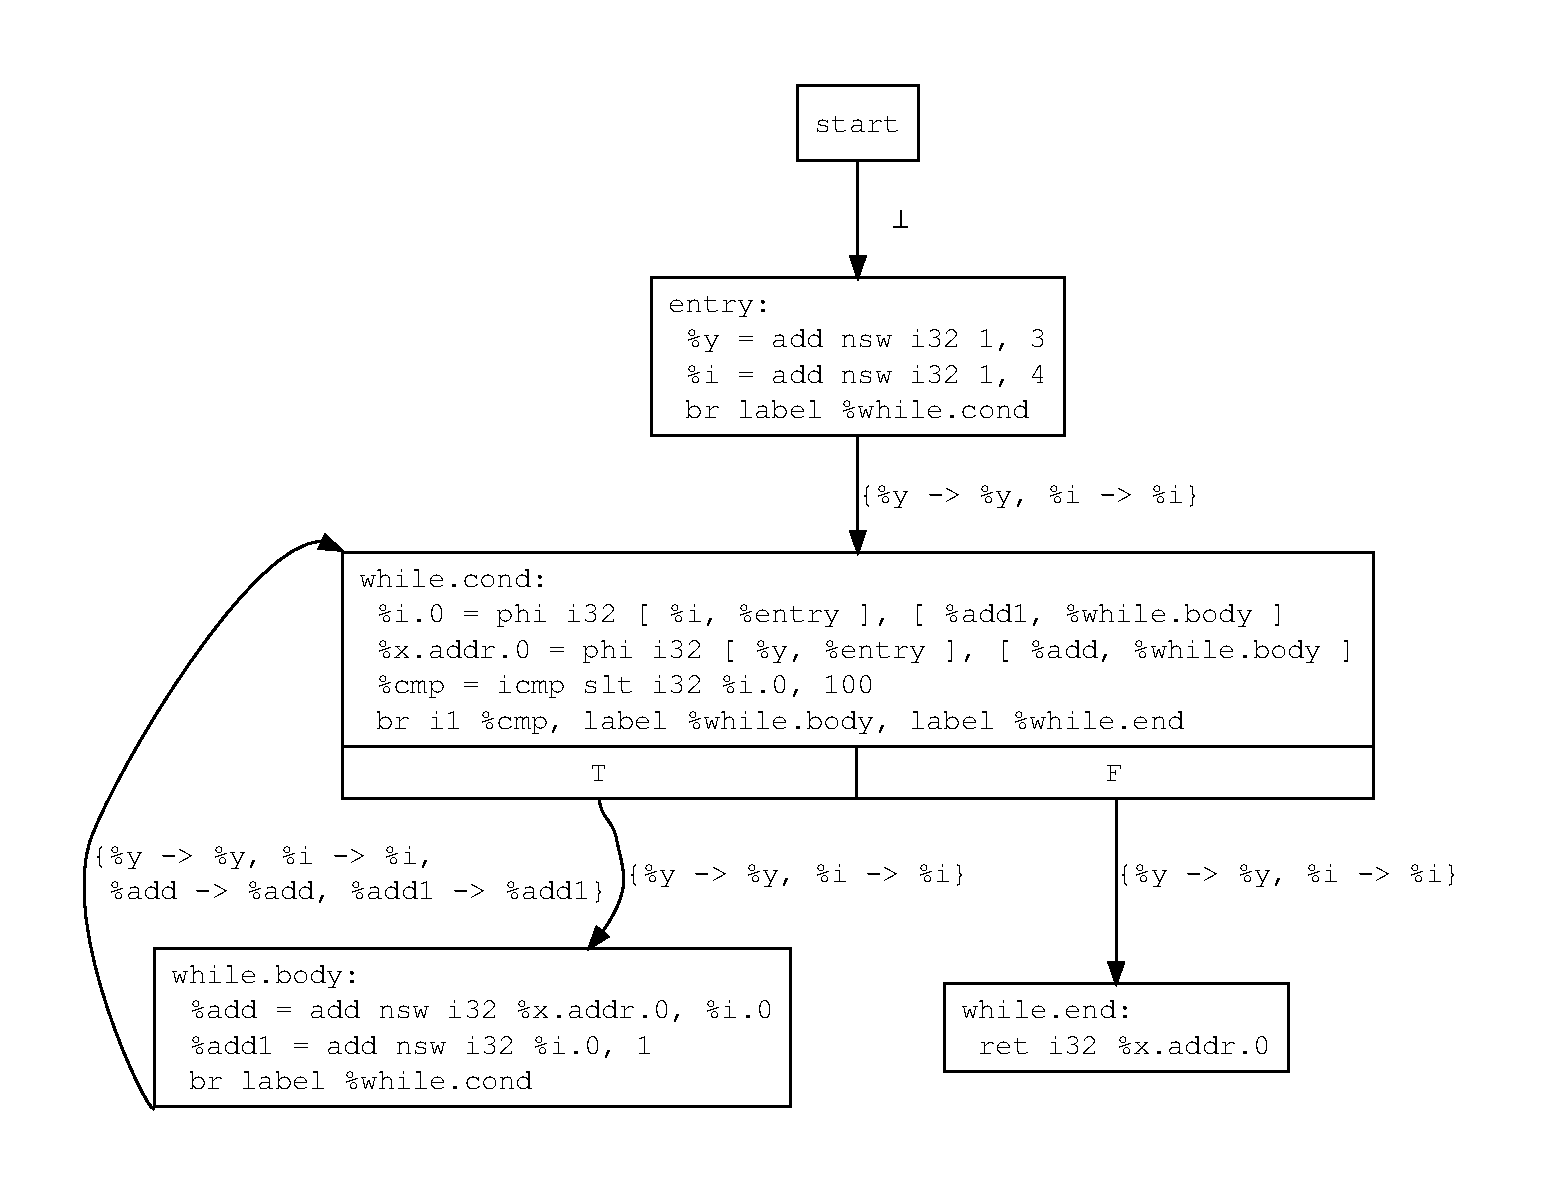
\includegraphics[scale=.4]{figures/cse/loop/loop-no-do-cse.pdf}
\subsection{Range Analysis}
\subsection{Intra-Procedural Pointer Analysis}

\subsection{Range Checking}

As per the assignment, we also implemented a range checking pass to make sure that array accesses remain inbound and raise warnings otherwise. This was fairly straightforward once the range analysis work was completed. To do this part, we simply ran our range analysis on the incoming function, then we scanned through the instructions for a getelementptr instruction. We then look at the lattice point at this instruction, query the index range, and raise a warning if it has a range that potentially falls outside of the range of the array.

\end{document}

